\section*{Exercice 145 -- Retard et PI}
\setcounter{exo}{0}
%CCMP PSI 2005


La consigne d’effort de freinage du train est modulée en fonction de la charge du train. Les ordinateurs
embarqués conjuguent le frein électrique et le frein mécanique sur les motrices. Le frein électrique est
prioritaire pour tout début de freinage à vitesse supérieure à \SI{15}{km.h^{-1}}; en dessous de ce seuil, le frein
mécanique devient indispensable. On s’intéresse dans cette partie au freinage mécanique uniquement.

Le freinage mécanique est réalisé par l’intermédiaire de blocs frein pneumatiques à semelles sur toutes les
roues, sauf le bogie équipé de la roue phonique. Le circuit de frein mécanique est piloté par une électrovalve
qui délivre vers le relais de pression une pression proportionnelle à son courant de commande. Ce relais de
pression autorise, dans la même proportion, le passage de l’air provenant du réservoir auxiliaire à
destination des blocs pneumatiques de freinage.

Sur la figure suivante se trouve reproduite l’évolution du couple de freinage mécanique en fonction du temps en
réponse à une tension unitaire délivrée par l’électrovalve. On note par la suite $C_f (t)$ cette évolution.

%\begin{obj}
%\end{obj}

\begin{center}
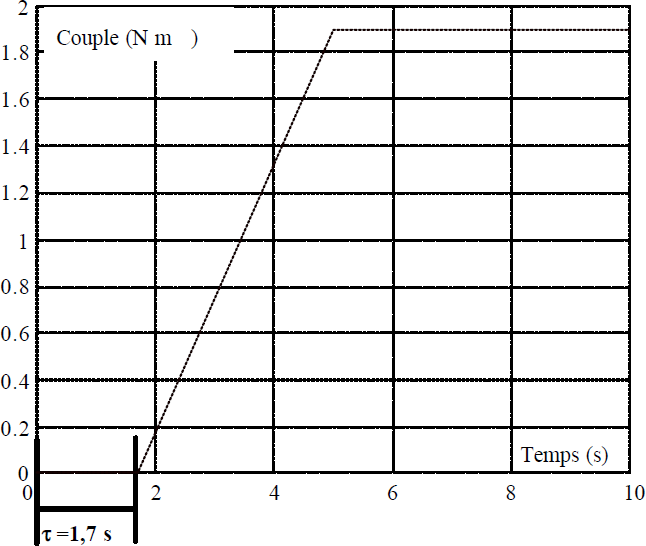
\includegraphics[width=\linewidth]{977_01}%
\end{center}

On constate que l’effet d’une demande de freinage initiée à l’instant $t = \SI{0}{s}$ ne se manifeste qu’à partir de
l’instant $t =\SI{1,7}{s}$ . Le temps $\tau = \SI{1,7}{s}$ est alors appelé retard pur du système.

\subparagraph{}
\textit{En décalant l’origine temporelle de la valeur du retard pur, déterminer la fonction de transfert
du frein $H'_{\text{frein}} ( p)$ approchée sous la forme d’un système du premier ordre : $H'_{\text{frein}} ( p) = \dfrac{K_f}{1+\tau_f p}$ où $K_f$ et $\tau_f$ seront déterminés à partir de la courbe de la figure précédente.}
\ifprof
\begin{corrige}
\end{corrige}
\else
\fi

\subparagraph{}
\textit{En déduire la fonction de transfert tenant compte du retard $H_{\text{frein}}( p)$. On donne la relation suivante entre la transformée de Laplace d’une fonction $x$ non retardée et la transformée de Laplace de cette même fonction avec un
retard $t_0$ : $\mathcal{L}\left( x(t - t_0)\right)= \mathcal{L}\left( x(t)\right)e^{-t_0 p}$.}
\ifprof
\begin{corrige}
\end{corrige}
\else
\fi

Le train étant sur une voie en pente, son poids induit un couple perturbateur $C_{\text{per}}(t)$. Le schéma-blocs global
de l’asservissement de l’accélération en phase de freinage mécanique est alors représenté figure suivante.
Dans un premier temps, le retard pur est négligé (le terme $e^{-1,7 p}$ n’est pas pris en compte). 

\begin{center}
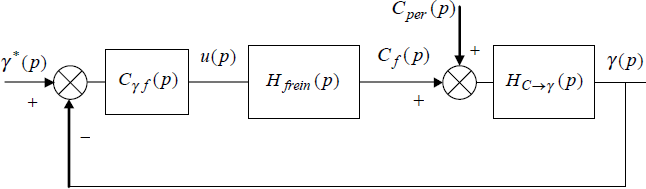
\includegraphics[width=\linewidth]{977_02}%
\end{center}

Un correcteur $C_{\gamma f}(p)$ de type P.I. (Proportionnel Intégral) a été élaboré avec cette hypothèse. On donne sur
le document-réponse le tracé dans le plan de Bode de la réponse fréquentielle du module et de la phase de
la fonction de transfert en boucle ouverte corrigée.

\begin{center}
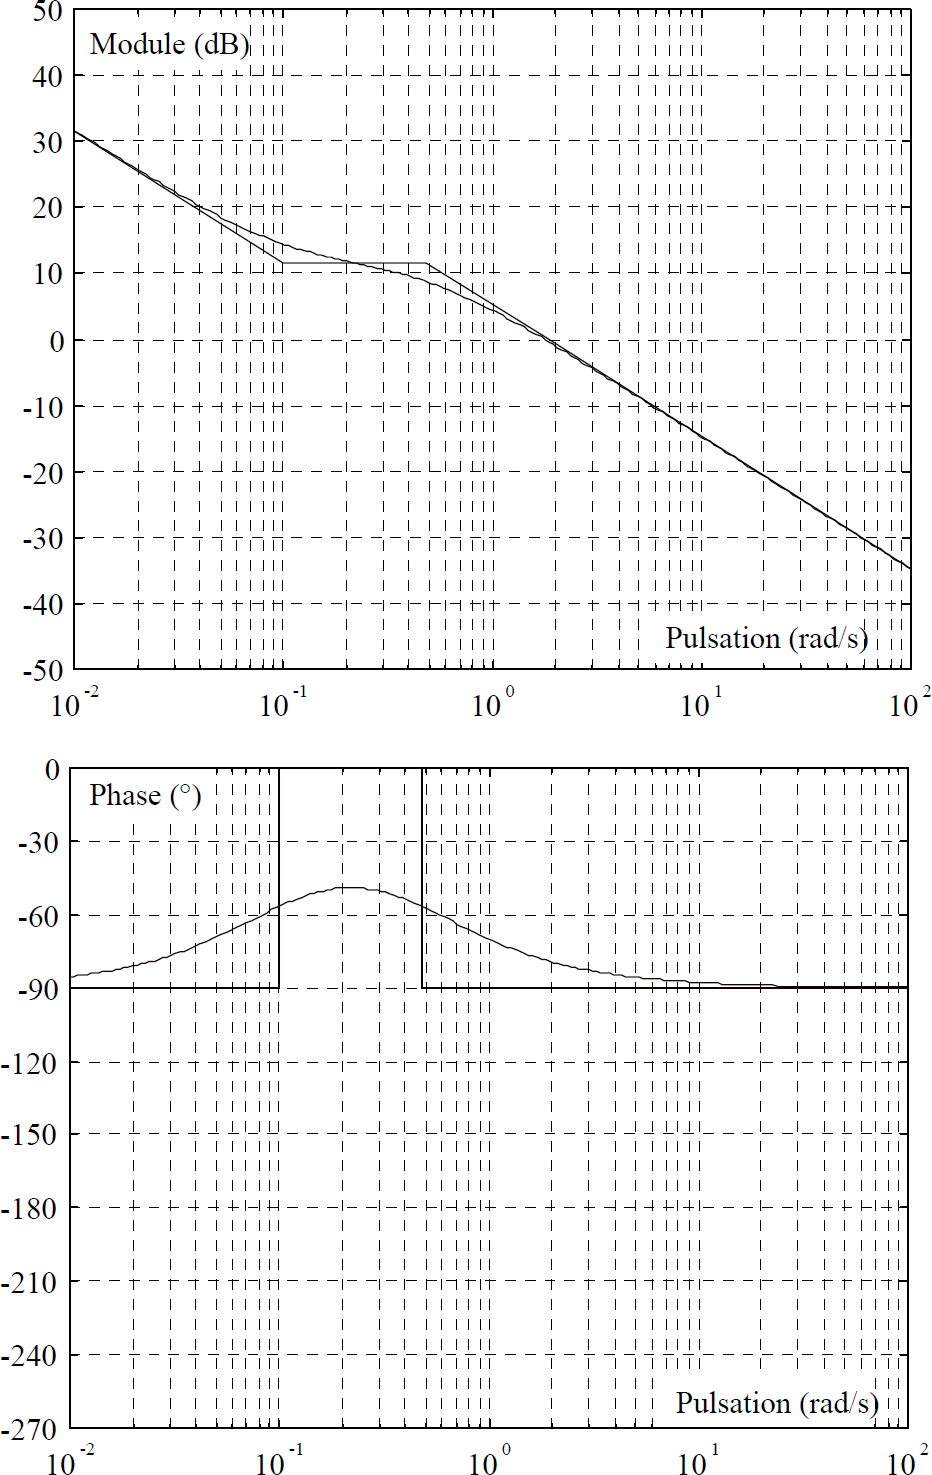
\includegraphics[width=\linewidth]{977_03}%
\end{center}



\subparagraph{}
\textit{Analyser les performances ainsi obtenues avec le correcteur P.I. (pulsation de coupure à
\SI{0}{dB} et marges de phase et de gain).}
\ifprof
\begin{corrige}
\end{corrige}
\else
\fi

On cherche désormais à évaluer l’influence du retard pur sur le comportement de l’asservissement.

\subparagraph{}
\textit{Compléter en bleu sur la figue le diagramme de Bode de la boucle ouverte
corrigée en ajoutant désormais l’influence du retard pur.}
\ifprof
\begin{corrige}
\end{corrige}
\else
\fi

\subparagraph{}
\textit{Analyser les performances ainsi obtenues avec le correcteur P.I. (pulsation de coupure à 0 dB et
marges de phase et de gain), en tenant compte du retard pur.}
\ifprof
\begin{corrige}
\end{corrige}
\else
\fi

\subparagraph{}
\textit{À partir de ces résultats, analyser l’impact du retard pur sur le comportement du système. Quelle(s)
modification(s) du correcteur proposez-vous pour tenir compte de ce retard pur ?}
\ifprof
\begin{corrige}
\end{corrige}
\else
\fi

\begin{enumerate}
\item $H'_{\text{frein}} ( p) = \dfrac{1,9}{1+3,3 p} $.
\item $H_{\text{frein}} ( p) = \dfrac{1,9}{1+3,3 p} e^{-1,7 p}$.
\item $M\varphi = 100\degres$ et $\omega_c = \SI{2}{rad.s^{-1}}$.
\item ...
\item $M\varphi = -180\degres$ et $\omega_c = \SI{2}{rad.s^{-1}}$ et $MG = \SI{-4}{dB}$.
\item ...
\end{enumerate}